
\documentclass[a4paper, oneside, 11pt]{report}
\usepackage{epsfig,pifont,float,multirow,amsmath,amssymb}
\newcommand{\mc}{\multicolumn{1}{c|}}
\newcommand{\mb}{\mathbf}
\newcommand{\mi}{\mathit}
\newcommand{\oa}{\overrightarrow}
\newcommand{\bs}{\boldsymbol}
\newcommand{\ra}{\rightarrow}
\newcommand{\la}{\leftarrow}
\usepackage{algorithm}
\usepackage{algpseudocode}
\usepackage{natbib}
\topmargin = 0pt
\voffset = -80pt
\oddsidemargin = 15pt
\textwidth = 425pt
\textheight = 750pt

\begin{document}

\begin{titlepage}
\begin{center}
\rule{12cm}{1mm} \\
\vspace{1cm}
{\large  CMP-7009A Advanced Programming Concepts and Techniques}
\vspace{7.5cm}
\\{\Large Project Report - 16 January 2020}
\vspace{1.5cm}
\\{\LARGE Simulating the activities of an Ant colony}
\vspace{1.0cm}
\\{\Large Group members: \\ Alvin Lu}
\vspace{10.0cm}
\\{\large School of Computing Sciences, University of East Anglia}
\\ \rule{12cm}{0.5mm}
\\ \hspace{8.5cm} {\large Version 1.0}
\end{center}
\end{titlepage}


\setcounter{page}{1}
%\pagenumbering{roman}
%\newpage


\begin{abstract}
An abstract is a brief summary (maximum 250 words) of your entire project. It should cover your objectives, your methodology used, how you implemented the methodology for your specific results and what your final results are, your final outcome or deliverable and conclusion. You do not cover literature reviews or background in an abstract nor should you use abbreviations or acronyms. In the remainder of the report the chapter titles are suggestions and can be changed (or you can add more chapters if you wish to do so). This template is designed to help you write a clear report but you are welcome to modify it (at your peril ...). Finally, a guideline in size is approximately 3,500 words (not including abstract, captions and references) but no real limit on figures, tables, etc.
\end{abstract}

\chapter{Introduction}
\label{chap:intro}

The biological world has always been a source of inspiration for computer models and algorithms. Within successful model developed, swarm intelligence have always been a topic of interest spanning across wide range of disciplines \citep{Swarm_Intro}. In computing, swarms are usually associated with ants that exhibits large amount of behaviours that can potentially be used to optimise algorithms. Whilst there exist techniques and simulations \citep{Ant_Simulator} \citep{Ant_Simulator_Revisited} \citep{Ant_Simulator_Intro}  that mimics the certain behaviour of ants, there aren't software available that simulate ants realistically in  the biological world.

This project aims to develop a realistic ant simulator that allows customisation of various biological settings to simulate different ant colonies in varying environments. It will provide a method to show an accurate representation of ant behaviours, simulate survivability or ants in different settings, and reveal emergent properties that may benefit future swarm intelligence.

\section{Report structure}
Chapter \ref{chap:intro} will provide an introduction to the topic which will be followed by chapter \ref{chap:background} that provides scientific background, previous materials and motivation of for the project. Chapter \ref{chap:design} will detail the design considerations for the solution, supported by analysis of previous literature and existing solutions. Implementation details will be explained in chapter \ref{chap:Implementation} showing figures of the solution and design modifications made. Chapter \ref{chap:Testing} will provide testing and evaluation of the final software with discussions on it's strengths and weakness and the report will end with chapter \ref{chap:conclusion} providing a conclusion to the project.

\chapter{Background}
\label{chap:background}
\section{Background information}
Swarming is a behaviour that is commonly found in social animal species \citep{Swarm_Animals}. The concept of swarming is having a large group of individually operating unit (agents or individual animal) working together to achieve a task that is typically to great for a unit to complete on its own \citep{Swarm_Explanation}. Large amount of research has been conducted to explain the evolutionary benefits of such behaviour and researchers are aiming to adapt some of these properties into various computer systems. This is commonly achieved by having a group relatively simpler agents that can communicate between each other instead of a singular system to complete tasks collectively by converging individual accomplishments \citep{Swarm_Properties}.

Within animals that exhibit swarming, ants are one of the insect that has been vigorously studied for their behaviour. Ants most commonly utilise swarming during the process of foraging. Certain species of ants are shown to leave pheromones to share information an individual ant has learnt \citep{Ant_Pheromones}. The two most common pheromones are home pheromones that can guide them home and also pheromones that guide other ants to food sources \citep{Ant_Pheromones}. The pheromones can vary in their duration and potency, which allows transfer of information such as recency and importance of the information \citep{Ant_Pheromones}. Aside from pheromones, ants are shown to retain memories of places it has seen, using visual cues to guide them to their destination \citep{Ant_Memory_1} \cite{Ant_Memory_2} \cite{Ant_Memory_3}.


\section{Existing methods}
Currently, an ant simulator was found publicly available online that uses the MASON simulation toolkit \citep{Mason}. The simulator provides a list of features listed below:
\begin{itemize}
	\item Allows customisation of certain values such as the ant population and evaporation rate.
	\item Allows pausing, playing and speeding up or slowing down the simulation.
	\item Shows the pheromone and ant data of a particular point in the map when clicked
\end{itemize}

The simulator provides quick and easy way to visualise movements of the ants however it the customisation was limited as the location of the hive, food and obstacle type can not be changed. This simulator aims only to show how ants eventually converge into a path from hive to food shown in figure \ref{MASON_Ant_Converged} which limits the flexibility of the simulator. The source code of the ant simulator is available on \textit{GitHub} for reference.

\begin{figure}[htb]
	%\begin{center}
	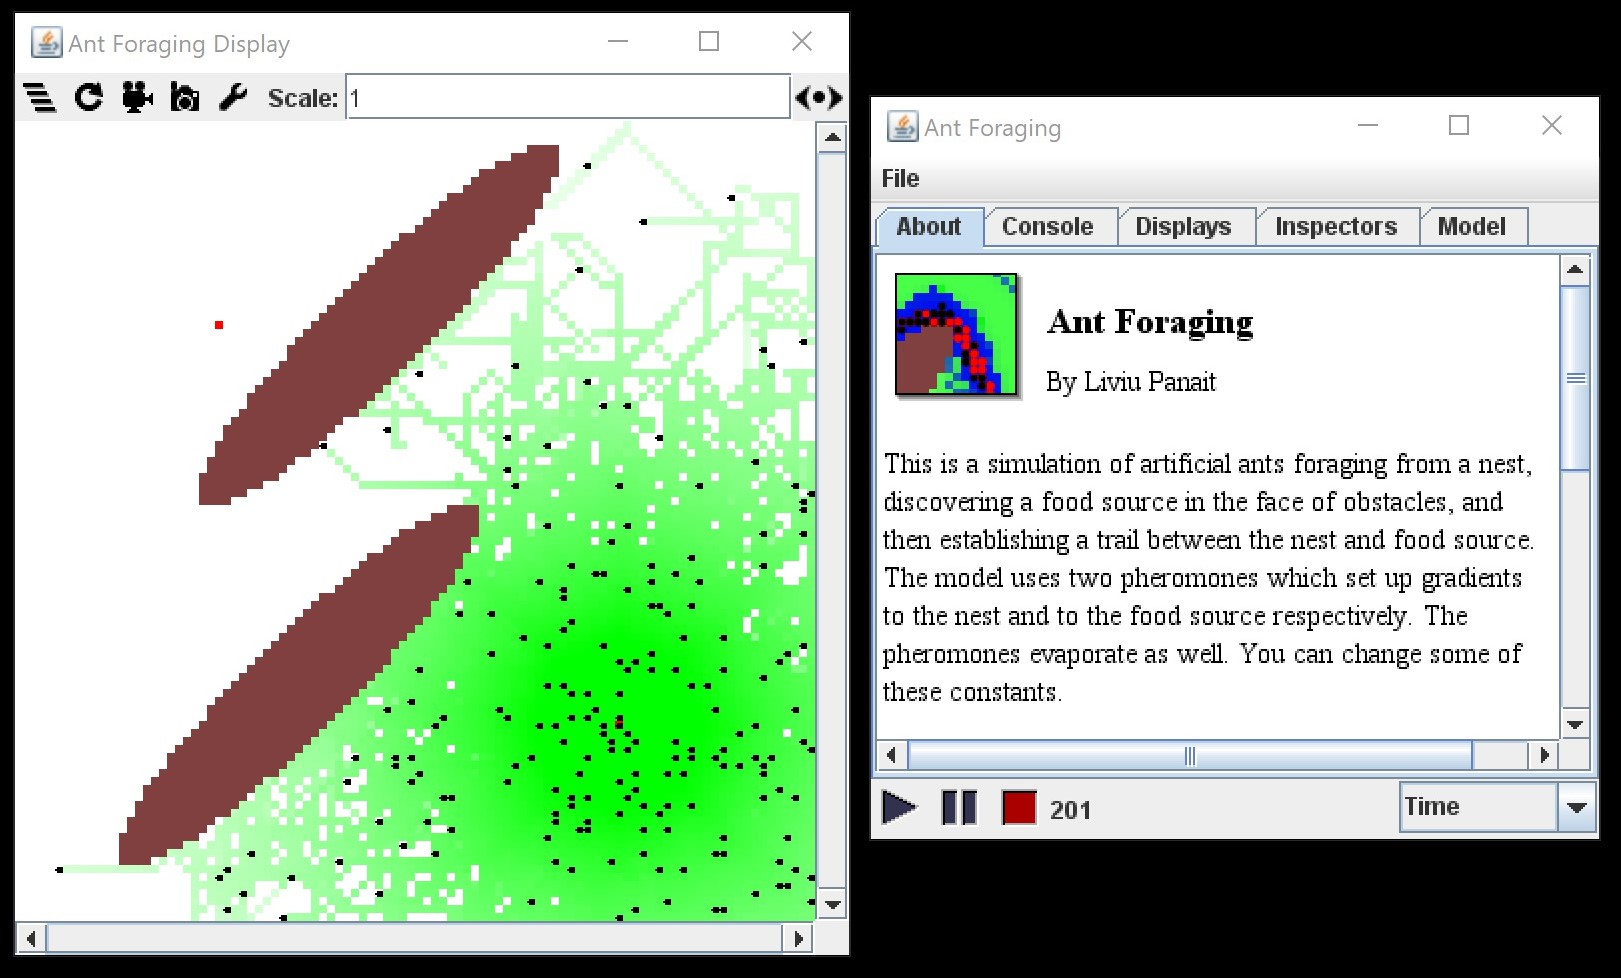
\includegraphics[width=1.0 \columnwidth]{MASON_Ant.jpg}
	\caption{Ant simulator developed by Liviu Panait \citep{Ant_Simulator}}
	\label{MASON_Ant}
	%\end{center}
\end{figure}

\begin{figure}[htb]
	%\begin{center}
	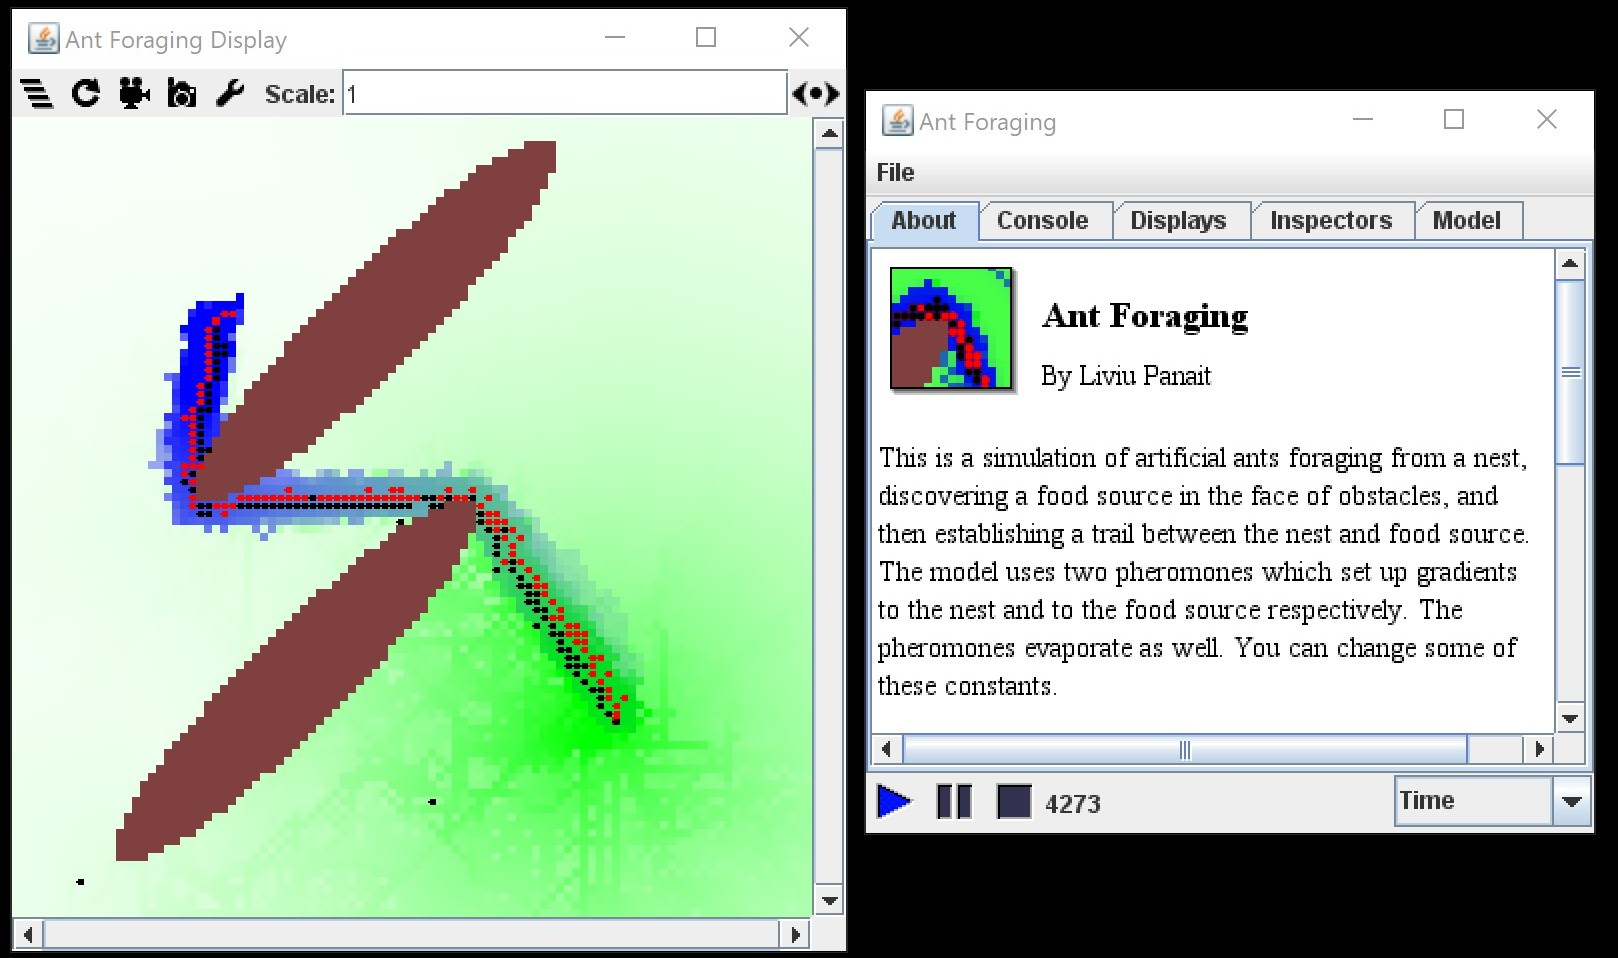
\includegraphics[width=1.0 \columnwidth]{MASON_Ant_Converged.jpg}
	\caption{Convergence of ant in the simulator \citep{Ant_Simulator}}
	\label{MASON_Ant_Converged}
	%\end{center}
\end{figure}

\chapter{Design}
\label{chap:design}
\section{MoSCoW}
\subsection{Must}
\begin{tabular}{|| p{3.5cm} | p{10.5cm} ||} 
	\hline
	Requirements & Description \\
	\hline
	Independent ant movements & Ants must move independently from each other \\
	\hline
	Creating hive & Allow creation of a hive. The hive will be the starting point of all ants belonging to that hive. \\
	\hline
	Static food & Allow creation of static food items on the map. \\
	\hline
	Pheromone types & Contain a pheromone system that allows deposition of pheromone values on the ground. \\
	\hline
	Pheromone evaporation & Deposited pheromones should decrease in concentration overtime in a fixed rate. \\
	\hline
	Obstacle creation & Able to create obstacles that ants can't move on or under \\
	\hline
	Ant births & Able to dynamically generate ants in with a given birth rate \\
	\hline
	Ant death & Ants will die and be removed from the map by probabilistic death rate \\
	\hline
	Pause and play simulation & Allow users to pause the running simulation and replay it multiple times \\
	\hline
	Shows ant data dynamically & Shows ant population and time elapsed on the UI dynamically  \\
	\hline
\end{tabular}

\subsection{Should}
\begin{tabular}{||p{3.5cm} | p{10.5cm} ||} 
	\hline
	Requirements & Description \\
	\hline
	Customisable hive location & The hive location of ants should be customisable on allowed locations on the map. \\
	\hline
	Customisable food location & Food items should be customisable on allowed locations on the map. \\
	\hline
	Customisable global evaporation rate & Rate of evaporation of pheromones can be customised\\
	\hline
	Reset simulation & Allows resetting the simulation with different values \\
	\hline
	Time scaling & Automatically scales the time to reflect realistic values. Allow users to enter actual values for attributes that are connected to time.\\
	\hline
\end{tabular}

\subsection{Could}
\begin{tabular}{|| p{3.5cm} | p{10.5cm} ||} 
	\hline
	Requirements & Description \\
	\hline
	Multiple hives & Allows creation of multiple ant colonies with varying population \\
	\hline
	Customizable terrain & Terrains can be customised by the users by painting pixels on the map \\
	\hline
	Moving food item & Allows creation of food item that moves across the screen \\
	\hline
	Predator & Allows creation of predators that attacks and consumes the ants\\
	\hline
	Customisable individual evaporation rate & Allows customisation of individual evaporation rates \\
	\hline
	Preset ant settings & Provides a list of settings that reflects actual values of ant species \\
	\hline
	Varying ant types & Allows creation of different types of ant within a colony \\
	\hline
	Pheromone data at point & Outputs the pheromone data of a particular point in the map\\
	\hline
	Creation of new pheromones & Allows creation of pheromones with different properties\\
	\hline
\end{tabular}

\subsection{Won't}
\begin{tabular}{|| p{3.5cm} | p{10.5cm} ||} 
	\hline
	Requirements & Description \\
	\hline
	Detailed UI models &  The UI of different items(sprites) in the simulator will not have detailed models and will be represented by simple shapes\\
	\hline
	In-built screen recording & The system will not provide recording features \\
	\hline
	Nupital flight simulation & The system will not simulate the process of nupital flight \\
	\hline
\end{tabular}

\section{Structure of the system}


\section{Ant movement AI}
All ants can move to the 8 potential directions shown in figure \ref{fig:Ant_Direction}. If there isn't any pheromone data found in their surroundings, the ants will move in random directions but they will prioritise the three direction that the ant is in front. 

During analysis of MASON ant simulator and literatures associated, It was found that the the ants in the simulator relies purely on pheromones for navigation  which might result in ants being stuck in in a cyclic movement if the food source is located further away from the hive where surrounding home pheromones may have evaporated or the density of ants are not high enough to ensure navigation back to the hive. Due to this, individual ants are designed to retain a set amount of locations that it has  recently visited and will avoid moving back to the locations unless necessary. 

Algorithm \ref{Algorithm:General} shows the high level movement pattern of ants. Algorithm \ref{Algorithm:Find_Home}, \ref{Algorithm:Home_Pheromone} and \ref{Algorithm:Home_Distance} shows the algorithm used for ants to find their way back to their hive when carrying food. Movement patterns when ants are following food pheromones to food source are similar to following home pheromones back to the hive.

\begin{figure}[htb]
	\begin{center}
	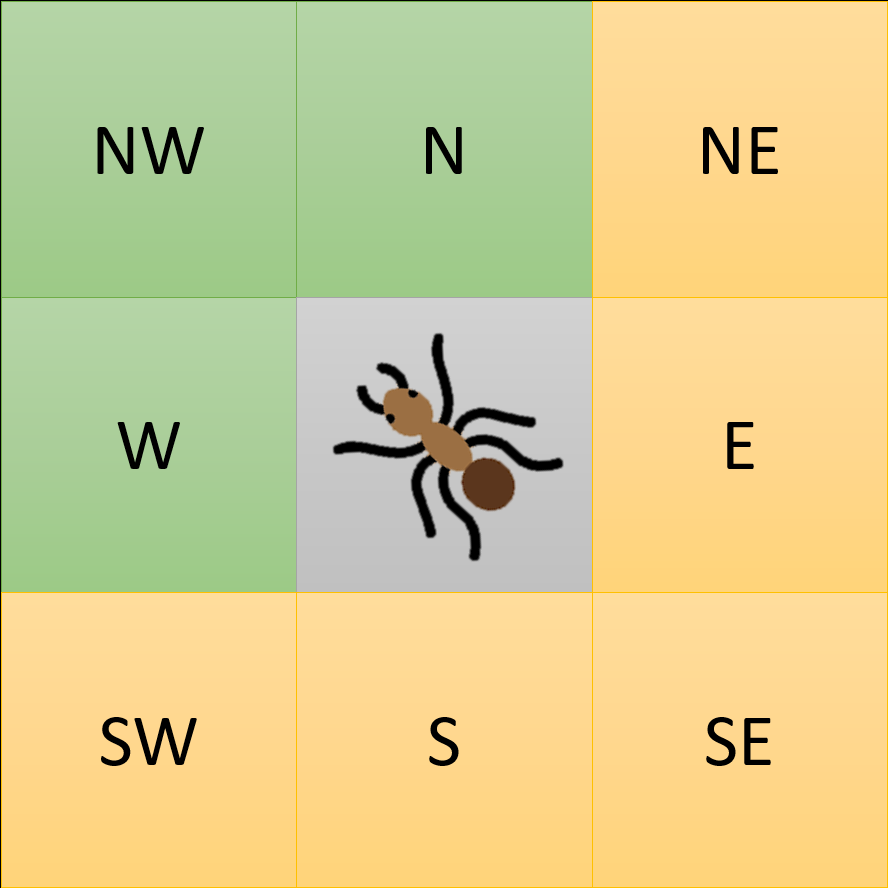
\includegraphics[width=0.35 \columnwidth]{Ant_direction.png}
	\caption{Directions an ant can move to if unobstructed. Ants will prioritise moving towards the three directions in front of them (Ant facing NW). Ant image sourced from \textit{Stockio}}
	\label{fig:Ant_Direction}
	\end{center}
\end{figure}

\begin{algorithm}[th]
\caption{ Ant foraging algorithm } \label{Algorithm:General}
\begin{algorithmic}[1] 
	\If{HasFoodItem}
		\State Find-Direction-Home
	\ElsIf{FoundFoodPheromone}
		\State Follow-Food-Pheromone
	\Else
		\State Random-prioritised-movement
	\EndIf
\end{algorithmic}
\end{algorithm}

\begin{algorithm}[th]
	\caption{ Find-Direction-Home algorithm}  \label{Algorithm:Find_Home}
	\begin{algorithmic}[1]
		\If{Ant reached the hive}
			\State Drop food 
			\State $HasFoodItem \gets False$
		\Else
			\State direction $\leftarrow$ Decide-Direction-Home-With-Pheromone
			\If{direction = NULL}
				\State direction $\leftarrow$ Decide-Direction-Home-Without-Pheromone
			\EndIf
		\EndIf
		\State moveAnt($direction$)
	\end{algorithmic}
\end{algorithm}

\begin{algorithm}[th]
	\caption{ Decide-Direction-With-Pheromone algorithm}  \label{Algorithm:Home_Pheromone}
	\begin{algorithmic}[1]
		\State potential-directions $\leftarrow$ \{ \}
		\While{there's possible directions}
			\If{direction is not blocked}
				\If{direction is closer to hive \& direction wasn't visited recently}
					\If{direction-contains-pheromone}
						\State potential-directions $\overset{+}{\leftarrow}$ direction
					\EndIf
				\EndIf
			\EndIf
		\EndWhile
		\If{potential-directions = NULL}
			\State return NULL
		
		\Else
			\State direction $\leftarrow$ direction-maximum-pheromone$(potential-directions)$
			\State return direction
		\EndIf
	\end{algorithmic}
\end{algorithm}

\begin{algorithm}[th]
	\caption{ Decide-Direction-Without-Pheromone algorithm}
	 \label{Algorithm:Home_Distance}
	\begin{algorithmic}[1]
		\State potential-directions $\leftarrow$ \{ \}
		\While{there's possible directions}
		\If{direction is not blocked}
			\If{potential-directions = NULL \& direction wasn't visited recently}
				\State potential-directions $\overset{+}{\leftarrow}$ direction
			\ElsIf{direction is closer to hive}
				\State potential-directions $\overset{+}{\leftarrow}$ direction
			\EndIf
		\EndIf
		\EndWhile
		\State direction $\leftarrow$ direction-closest-to-home$(potential-directions)$
		\State return direction
	\end{algorithmic}
\end{algorithm}

\chapter{Implementation}
\label{chap:Implementation}
\section{Platform and packages}
The simulator is developed in Java using the IDE \textit{IntelliJ}. Using Java as the development language ensures that the solution can be run on a wide range of Operating Systems while the object-oriented paradigm allows definition of classes that's duplicable and inheritable. This would be beneficial for this project as the simulator involves creation of large amount of objects that are similar structurally but has to behave independently. The UI will also be developed using \textit{JavaFX} as its platform. JavaFX provides the ability to separate UI from the implementation logic using FXML. It allows quick development of simple user interface that can be easily expanded and updated as JavaFX also supports CSS and HTML.


\begin{table}[h]
\caption[]{Original diameters and diametral strains as reported by
  Sorbe and Dahlgren \cite{Sorbe:1983} (columns 1-2), from a previous 
  experiment by Lapeer and Prager and reported in \cite{Lapeer:2001}
  (columns 3-4), and from the current experiment (columns 5-6).}
\begin{center}
\begin{tabular}{|l|c|c||c|c||c|c|}\hline
& \multicolumn{2}{c||}{S-D} & \multicolumn{2}{c||}{L-P old} & \multicolumn{2}{c|}{L-P new} \\ \hline
Diameter & length & strain & length & strain & length & strain \\ \hline
$\mi{MaVD}$ & 140.5 & +1.90 & 129.3 & +0.30 & 129.3 & +1.43 \\
$\mi{OrOD}$ & 131.4 & +0.10 &   -   &  -    & 119.9 & +1.85 \\
$\mi{OrVD}$ & 126.9 & +2.20 & 119.3 & +0.25 & 119.3 & +1.24 \\
$\mi{OFD}$  & 134.0 & +0.40 &  -    &   -   & 119.7 & +1.82 \\ 
$\mi{SOFD}$ &  -    &   -   &  -    &   -   & 113.2 & -0.85 \\
$\mi{SOBD}$ & 117.1 & -1.70 &  88.7 & -1.07 &  88.7 & -2.52 \\
$\mi{BPD}$  & 105.0 &  0.00 &  89.7 & -0.21 &  89.7 & -0.83 \\ \hline
\end{tabular}
\label{Res01}
\end{center}
\end{table}

Note that code snippets or lists of crucial programming code or large UML diagrams should go in the Appendix/Appendices.


\chapter{Testing and Discussion}
\label{chap:Testing}
As the software depends heavily on the ants interaction with the environment, testing will be conducted heavily towards the end of the development stage instead of early stages. Bugs and issue are predicted to be mostly emergent, caused by the ants interaction with its environment.

\section{Unit testing}
For unit testing, a test class was created within the package to test advanced method implemented in all classes. Values that are passed to and object are checked using console output to print out the values.

\section{Integration testing}
parameter passing

\section{User testing}

\chapter{Conclusion and Future Work}
\label{chap:conclusion}
Conclude your achievements and put them in perspective with the MoSCoW analysis you did early on. Be honest by declaring for example S categorised objectives which did not make it to the final deliverable rather than reversely modifying your MoSCoW in Chapter \ref{chap:intro}! Also discuss future developments and how you see the deliverable improving if more time could be spent. Do not put in subjective opinions or rants or excuses as to why something did not work out as planned in your report. A technical report is not a medium for complaints as there are other outlets for that typically well before you came to this stage (e.g. labs, e-mail etc.).


\bibliographystyle{unsrt}
\bibliography{References}

\chapter*{Appendix A}

Put in tables of data or protocols (e.g. for testing) or code listings or UML diagrams which may take up several pages and do not sit well in the main body text.

\end{document}

